\chapter{Proposed phase recovery architecture} \label{Proposed phase recovery architecture}

% \section{System overview}
% \todo{explain what the purpose is of the 2 stage design, e.g; why SBPS needs to track middle phase, SE the spread}

% Assumption that
% \begin{equation}
%     \sum_{i=0}^{B-1}\phi_i \ll 2\pi \Delta f T_s B
% \end{equation}


% \section{Serialized blind phase search}\todo{needs to be more detailed}
% The purpose of SBPS is to estimate the carrier phase of the middle of a processing block with 
% much lower complexity than conventional blind phase search. This estimate should be accurate enough to serve as the central 
% anchor point of the proposed phase recovery architecture, and must be in range of the largest CFO error that is possible
% for a certain frequency recovery architecture\todo{maybe explain why?}. 
% However, because only one phase estimate is produced per block 
% and because the BPS metric is inherently $\pi$/2-ambiguous for square QAM constellations, additional processing is required to 
% (i) track phase continuity between successive blocks and (ii) reconstruct the phase evolution inside the block. 
% These two tasks are handled by the phase unwrapping and spread estimation blocks, respectively.
% \\\\
% In conventional BPS, many candidate phases are evaluated in parallel over the full search interval (as 
% mentioned in section \ref{background: blind phase search}). 
% Although this leads to robust phase estimation, it also results in a substantial computational cost. \todo{maybe here 
% delve into the specific costs}
% \\\\
% For square \ac{QAM} constellations, the search interval is limited to
% \[
% \left[-\frac{\pi}{4},\frac{\pi}{4}\right),
% \]
% The key idea of \ac{SBPS} is to approximate the optimal test phase through successive refinement. 
% Instead of testing many candidate phases simultaneously, only two candidate rotations are evaluated at 
% each stage: one on either side of the current estimate. The candidate producing the lower decision-directed 
% metric is retained, after which the search interval is halved and a more refined correction is tested in the next stage.

% \begin{figure}[h]
% \centering
% 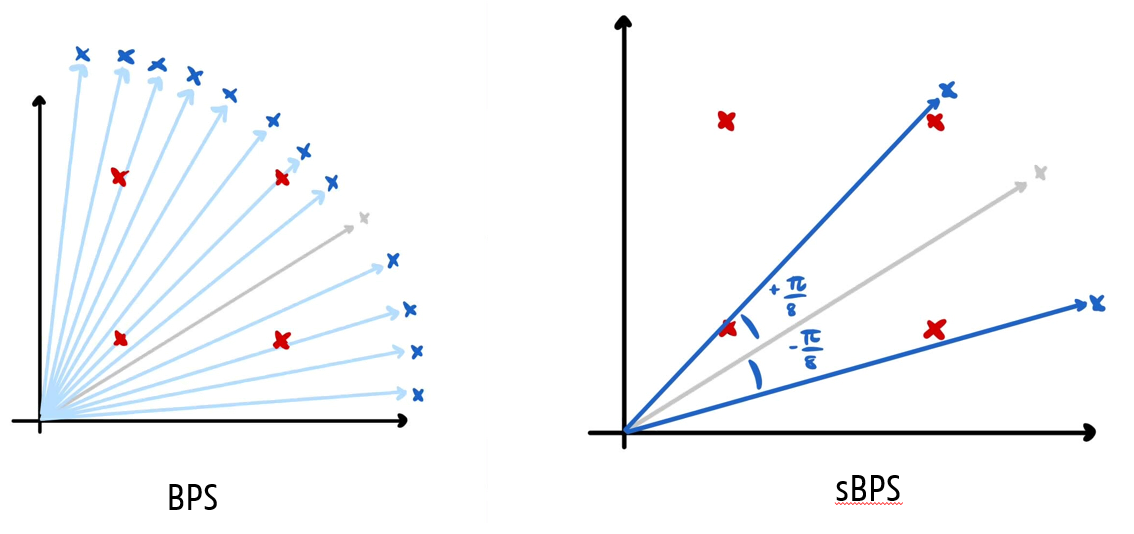
\includegraphics[width=0.8\linewidth]{figures/BPS_vs_SBPS.png}
% \caption{BPS versus SBPS guided phase estimation}
% \end{figure}
% \todo{remake figure for more fitting representation}

% In the binary variant adopted here \todo{motivate why binary search is chosen?}, the first stage tests the two hypotheses
% \[
% \phi_1 \in \left\{-\frac{\pi}{8},+\frac{\pi}{8}\right\},
% \]
% and stage \(m\) refines the estimate by adding or subtracting a correction term of magnitude \(\pi/2^{m+2}\). Hence, the estimate after 
% stage \(m\) can be written recursively as
% \[
% \hat{\phi}_m = \hat{\phi}_{m-1} \pm \frac{\pi}{2^{m+2}}.
% \]
% \\\\


% This staged procedure is equivalent to a binary search over the phase interval and yields an exponentially decreasing phase quantization error 
% as the number of stages increases. The referenced work formulates this refinement explicitly and 
% shows that the worst-case estimation error decreases with each added stage, while the number of candidate rotations only grows 
% linearly with the number of stages \cite{Jonas}. \todo{maybe useful to explain how complexity scales with accuracy} 
% \\\\
% For each candidate phase \(\phi\), a decision-directed metric is computed over a block of received symbols:
% \[
% J(\phi)=\sum_{k\in\mathcal{W}}\left|D\!\left(r_k e^{-j\phi}\right)-r_k e^{-j\phi}\right|^2,
% \]
% where \(r_k\) denotes the received symbol, \(D(\cdot)\) the slicer, and \(\mathcal{W}\) the symbol window 
% used for metric accumulation. 
% \begin{figure}[h]
% \centering
% 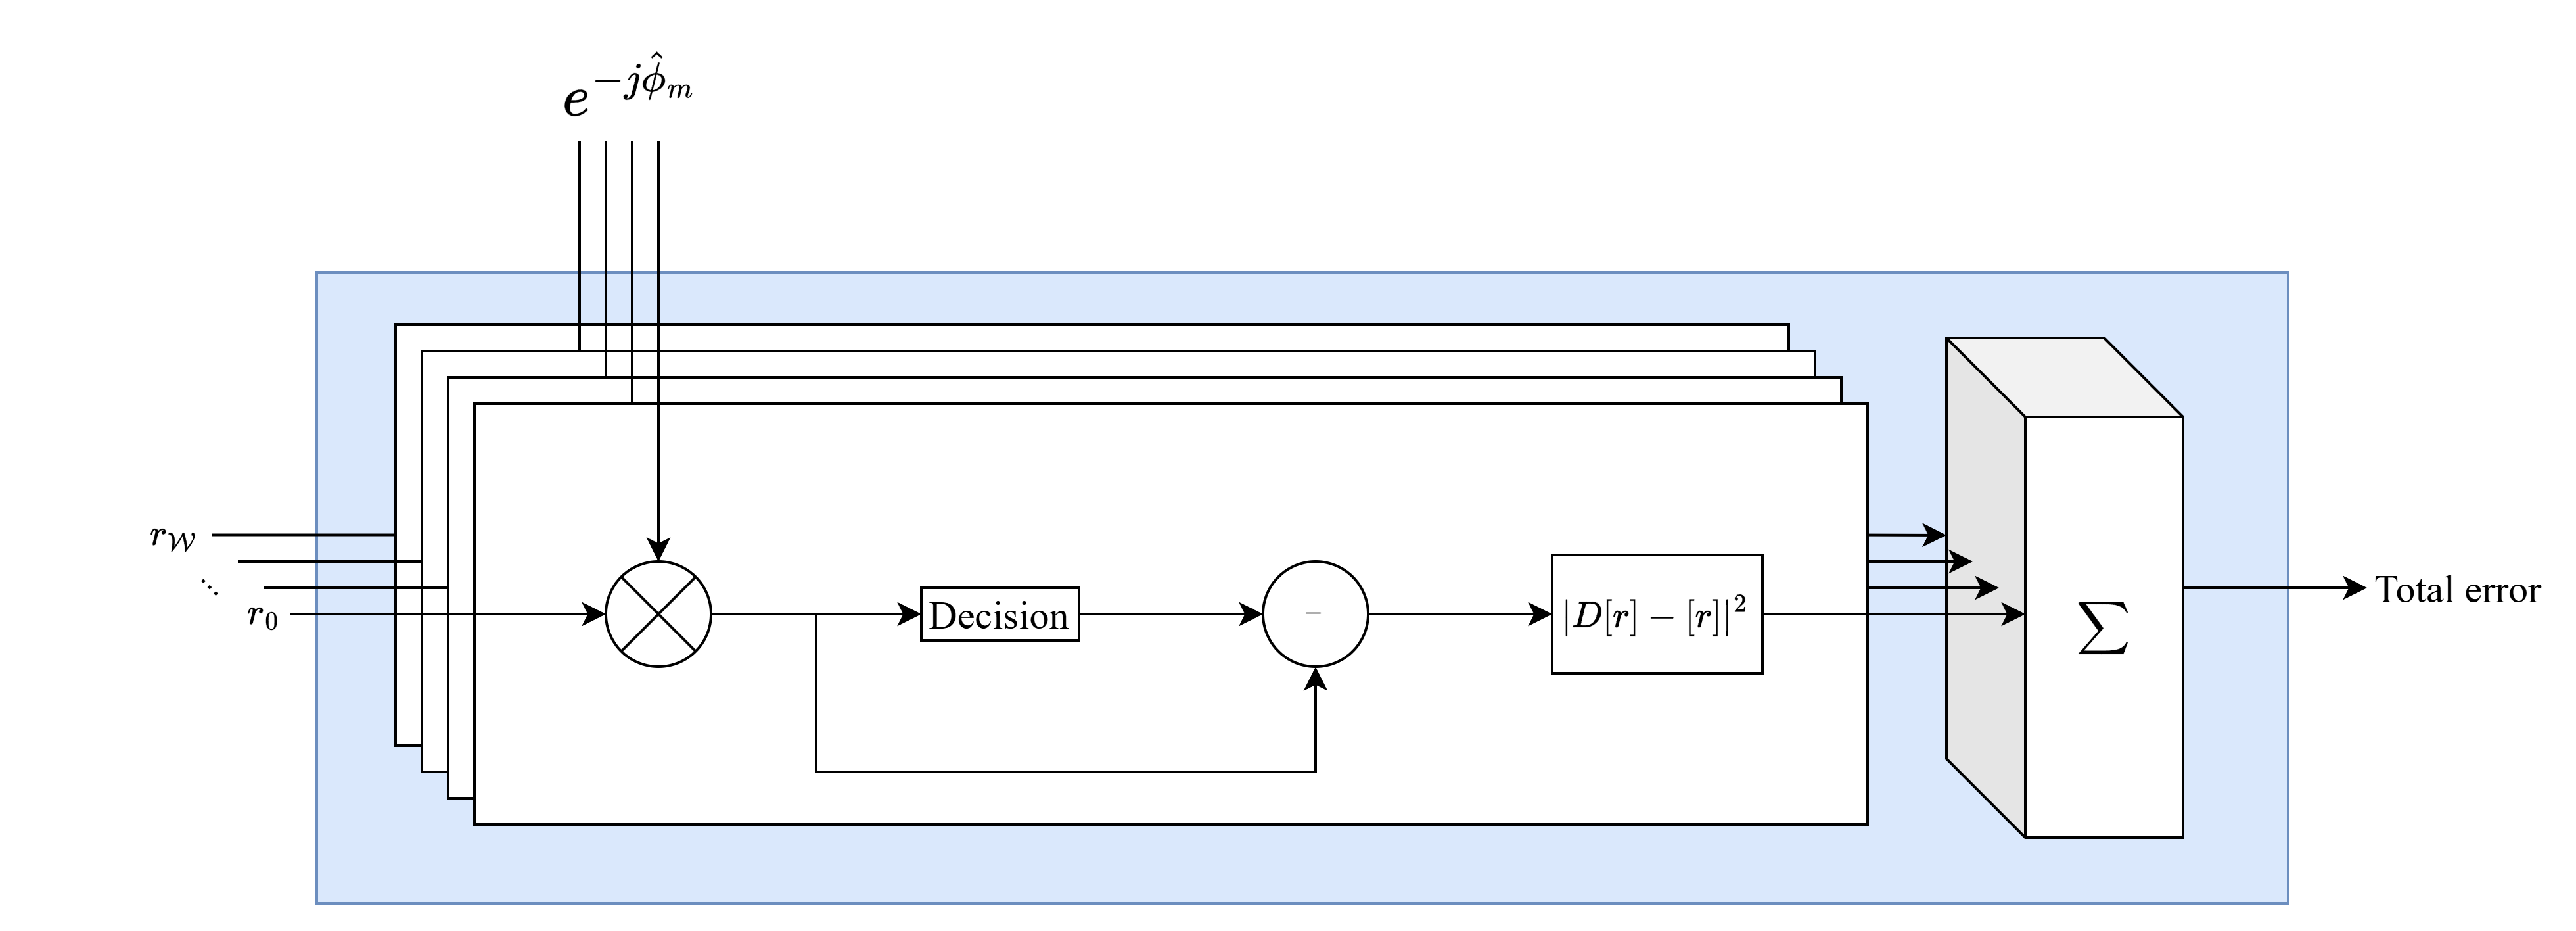
\includegraphics[width=0.9\linewidth]{figures/decision-directed_carrier_recovery.png}
% \caption{remake figure for more fitting representation}
% \label{fig:decision-directed_carrier_recovery}
% \end{figure}
% \todo{remake figure for more fitting representation}

% The candidate phase yielding the smallest metric is assumed to correspond most 
% closely to the true carrier phase. In this work, the resulting estimate is interpreted as the carrier phase at 
% the middle of the block, denoted by \(\hat{\phi}_e\). This interpretation is important, since in the presence of 
% residual frequency offset the carrier phase is not constant over the entire block but varies approximately linearly 
% with symbol index \todo{and laser phase drift is also present! (job of SE)}.
% \\\\
% \subsection{Adaptation to 16QAM}

% \subsection{Block size consideration}
% A consideration for the effectiveness of the SBPS is the frequency recovery stage \ac{FFT}-bin spacing. 
% This FFT bin spacing determines the maximum residual \ac{CFO} that remains after course frequency recovery 
% (equation \ref{eq: frequency recovery bin size error}).
% \\ 
% This residual CFO causes a phase drift across one SBPS processing block of $ B $ symbols:

% $$
%     \Delta \phi_{block} \approx 2\pi \Delta f_e B T_s
% $$

% Since $ T_s = 1/F_s $, subsituting the worst-case residual CFO gives:
% $$
%     \Delta \phi_{block,max} = 2\pi(\frac{F_s}{2N_{FFT}})B(\frac{1}{F_s})
% $$

% which simplifies to:

% $$
%     \Delta \phi_{block,max} = \pi \frac{B}{N_{FFT}}
% $$

% So, the worst-case accumulated phase drift over a block depends only on block size and FFT, not directly on sampling frequency.

% For the proposed SBPS with a $ \pi/4 $ unwrapping threshold, the following condition needs to be specified:

% $$
%     \Delta \phi_{block,max} \le \pi/4
% $$

% which gives

% \begin{equation}
%     N_{FFT} > 4B
% \end{equation}

% For example, a blocksize of $ B = 64 $ would need at least $ N_{FFT} > 256 $ for the SBPS to be effective without introducing (additional) cycle slips. 
% This is a theoretical minimum, and in practice a margin
% is recommended because of the presence of linewidth-induced phase noise and estimation errors. \todo{find ref for binsize related to accuracy?}
% \\\\
% Further, the block size has a dual effect on estimation quality. On the one hand, using more symbols in the metric accumulation 
% improves robustness against additive noise, because the random perturbations introduced by noise and symbol decisions are 
% averaged over a larger number of samples \cite{Mello_2018}. On the other hand, a larger block spans a longer time interval, so the phase variation 
% caused by residual frequency offset and phase noise becomes larger within the block. As a result, a single phase estimate 
% becomes less representative for all symbols in the block. 
% \\\\
% This trade-off is one of the main motivations for the proposed two-part 
% architecture: \ac{SBPS} provides an accurate estimate of the middle-block phase, while the spread estimation block reconstructs 
% the phase evolution around that midpoint.


% %-----------------------------------------
% % SPREAD ESTIMATION
% %-----------------------------------------

% \section{Spread estimation algorithm}
% As discussed in Sections~\ref{phase noise and frequency offset} and~\ref{carrier recovery in DSP chains}, 
% the residual impairments after coarse frequency recovery consist of both stochastic laser phase 
% noise and a remaining carrier frequency offset. While the residual phase drift caused by the laser 
% linewidth behaves as a random Wiener process, the remaining frequency offset introduces an approximately 
% linear phase ramp across a processing block (as seen in Figure~\ref{fig:linear_approx}). 

% The proposed \ac{SBPS} architecture estimates only a single carrier phase per block, namely the phase 
% located near the middle of the block. This estimate is sufficiently accurate to serve as a robust phase 
% reference for the block as a whole, but it does not describe how the phase evolves within the block itself. 
% As a result, directly compensating all symbols using only the middle-block phase estimate still leaves a 
% residual phase error on symbols located further away from the block centre.

% This effect becomes increasingly important when:
% \begin{itemize}
%     \item the residual \ac{CFO} after frequency recovery becomes larger,
%     \item the processing block size increases,
%     \item or the laser linewidth introduces additional phase drift.
% \end{itemize}

% Figure~\ref{fig:SBPS-versus-SBPS_and_SE} illustrates this effect. Although the middle of the block is 
% compensated correctly, symbols towards the edges of the block still exhibit residual constellation 
% rotation due to the remaining phase noise.

% \begin{figure}[H]
% \centering
% 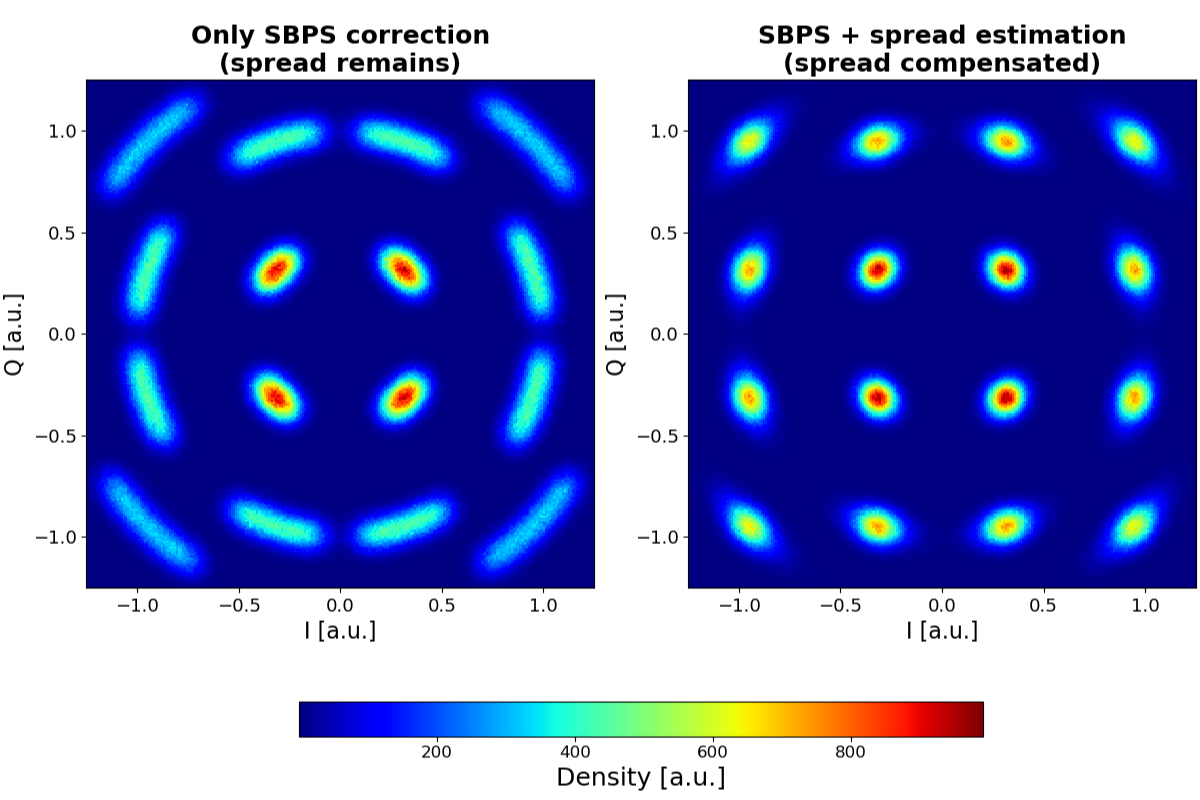
\includegraphics[width=0.8\linewidth]{figures/SBPS_versus_SBPS+SE_correction.png}
% \caption{SBPS versus SBPS+SE correction}
% \label{fig:SBPS-versus-SBPS_and_SE}
% \end{figure}

% % this should be said in the System overview section:
% The spread estimation (\ac{SE}) block is introduced to estimate this residual phase evolution 
% across the block. Rather than estimating a separate carrier phase for every symbol 
% which would significantly increase computational complexity, the proposed method estimates 
% the total phase spread over the block and reconstructs the intermediate phase trajectory from 
% this information.


% Under practical coherent datacenter operating conditions, the residual \ac{CFO} after coarse 
% frequency recovery is typically much larger than the phase variation caused by laser linewidth 
% over the duration of a single processing block. Therefore, the accumulated phase variation 
% inside the block may be approximated as locally linear:

% \begin{equation}
% \sum_{i=0}^{B-1} \phi_i \ll 2\pi \Delta f T_s B
% \label{eq:SE-linear-assumption}
% \end{equation}

% with $B$ the block size, $\phi_i$ the phase-noise contribution of symbol $i$, $\Delta f$ 
% the residual carrier frequency offset and $T_s$ the symbol period.

% Under the assumption that the accumulated phase variation inside the block is approximated as locally linear (Equation~\ref{eq:SE-linear-assumption}), the phase evolution across the block can be approximated by a nearly 
% linear slope, allowing the total phase spread to be estimated from only a limited number of
%  representative symbols.

%  \todo{explain more how modulation is removed when raising to the fourth power and only
% underlying phase evolution is left over}
% The proposed spread estimation algorithm operates on symbols that are raised to the fourth power. 
% For square \ac{QAM} constellations, the fourth-power operation suppresses the modulation-dependent 
% phase terms while preserving the carrier-related phase rotation. The resulting transformed 
% constellation therefore mainly contains information related to the underlying carrier phase evolution.

% % not really needed?
% % \begin{figure}[H]
% % \centering
% % \includegraphics[width=0.45\linewidth]{figures/fourth_power_constellation.png}
% % \caption{Illustration of a 16QAM constellation after fourth-power transformation}
% % \label{fig:fourth-power-constellation}
% % \end{figure}



% For a received symbol:

% \begin{equation}
% r_k = a_k e^{j\phi_k}
% \end{equation}

% the fourth-power operation gives:

% \begin{equation}
% r_k^4 = a_k^4 e^{j4\phi_k}
% \end{equation}

% The modulation phase ambiguity is removed because the phase states of square \ac{QAM} 
% constellations are rotationally symmetric over multiples of $\pi/2$. After fourth-power 
% transformation, the dominant remaining phase term corresponds to four times the carrier phase.

% \todo{tie in the definition of repr. symbols due to fourth power causing middle ring symbols 
% to become ambiguous, while inner and outer ring symbols maintain unambiguous}

% The spread estimation block uses representative symbols from different regions of the block:
% \begin{itemize}
%     \item one near the beginning of the block,
%     \item one near the middle,
%     \item and one near the end.
% \end{itemize}

% The first and last symbols are primarily used to estimate the magnitude of the phase spread, 
% while the middle symbol assists in determining the direction of the phase evolution.

% Let $R_0$ and $R_{B-1}$ denote the selected fourth-power symbols near the beginning and end
% of the block. The cosine of the total phase spread may then be estimated using the normalized dot product:

% \begin{equation}
% \frac{\langle R_0,R_{B-1}\rangle}
% {\|R_0\|\|R_{B-1}\|}
% =
% \cos(4|\theta|)
% \label{eq:spread-cos}
% \end{equation}

% with $\theta$ the total phase spread across the block.

% The spread magnitude can therefore be recovered through:

% \begin{equation}
% |\theta| =
% \frac{1}{4}
% \arccos
% \left(
% \frac{\langle R_0,R_{B-1}\rangle}
% {\|R_0\|\|R_{B-1}\|}
% \right)
% \label{eq:spread-mag}
% \end{equation}

% The use of $\arccos(\cdot)$ instead of $\arctan(\cdot)$ is important. Since the total phase 
% spread may exceed $\pi$, directly estimating the angle through an arctangent-based method 
% could lead to sign ambiguities and incorrect unwrap decisions. The cosine-based formulation 
% instead estimates only the absolute spread magnitude, after which the spread direction is 
% estimated separately.

% To determine the direction of the phase evolution, a second estimate is performed using symbols 
% from the beginning and middle of the block. The sign of the phase evolution can be obtained 
% through the sign of the complex cross product:

% \begin{equation}
% \mathrm{sign}(\gamma)
% =
% -\mathrm{sign}
% \left(
% \Re\{R_0\}\Im\{R_b\}
% -
% \Im\{R_0\}\Re\{R_b\}
% \right)
% \label{eq:spread-sign}
% \end{equation}

% with $a_b$ the selected middle-region symbol.

% Combining both estimates yields the final spread estimate:

% \begin{equation}
% \hat{\theta}
% =
% \mathrm{sign}(\gamma)
% \cdot
% |\theta|
% \label{eq:spread-final}
% \end{equation}

% The estimated spread is subsequently used in two different ways:
% \begin{enumerate}
%     \item to extrapolate leading and lagging phases for the phase unwrapper,
%     \item and to reconstruct multiple phase estimates inside the block during phase compensation.
% \end{enumerate}

% In this way, the spread estimation block effectively increases the frequency tracking 
% range of the overall carrier recovery system without requiring significantly more 
% \ac{SBPS} stages or a more accurate coarse frequency recovery stage.

% The method nevertheless introduces several limitations specific to square 16QAM 
% constellations. Unlike \ac{QPSK}, where the fourth-power operation maps all symbols 
% onto a single radius, the fourth-power transformation of 16QAM results in multiple 
% amplitude rings. Some transformed constellation points therefore become unsuitable 
% for accurate spread estimation because their relative phase relationships introduce 
% ambiguities.

% As a consequence, not every received symbol may be used directly for spread estimation. 
% The architecture therefore includes an input-selection stage that identifies suitable 
% candidate symbols before the actual spread calculation is performed. This selection
% procedure is discussed in the following subsection.

% \subsection{Input symbol consideration}\label{input selector}

% For \ac{QPSK}, the fourth-power operation maps all constellation symbols onto a single 
% circle. In the case of square 16QAM, however, the transformed symbols occupy multiple 
% radii after the fourth-power operation. This behaviour is illustrated in 
% Figure~\ref{fig:fourth-power-constellation}.

% \begin{figure}[H]
% \centering
% 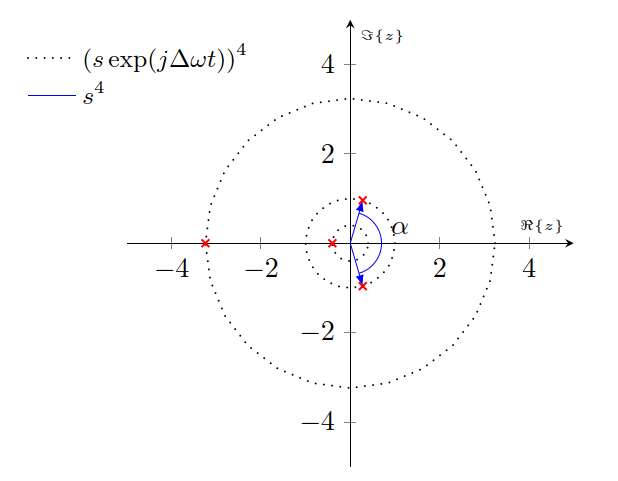
\includegraphics[width=0.45\linewidth]{figures/symbols_to_fourth_power.png}
% \caption{16QAM symbols to the fourth power}
% \label{fig:fourth-power-constellation}
% \end{figure}
% \todo{find a more fitting picture}

% As a consequence, some transformed constellation points become unsuitable for reliable 
% phase-spread estimation. In particular, symbols originating from the middle ring of the 
% 16QAM constellation can introduce large phase ambiguities after fourth-power transformation. 
% Using such symbols directly in the normalized dot-product calculation of (\ref{eq:spread-cos}) 
% can therefore lead to incorrect spread estimates.

% To mitigate this problem, the spread estimator only considers symbols originating 
% from the inner and outer constellation rings. Since these symbols retain an unambiguous 
% phase transformation after the fourth-power calculation, they yield more 
% reliable spread estimates.

% Rather than searching the complete processing block for suitable symbols, only a limited 
% subset of symbols near the beginning, middle and end of the block is evaluated. This 
% reduces hardware complexity while still maintaining a sufficiently high probability of 
% finding valid candidate symbols.

% Let $N$ denote the number of candidate symbols evaluated per region. Assuming uniformly 
% distributed 16QAM symbols, the probability of finding at least one valid candidate pair 
% may be approximated by:

% \begin{equation}
% P(\mathrm{hit})
% =
% 1 -
% \left[
% \left(
% \frac{1}{2^N}
% \right)^2
% +
% 2
% \left(
% \frac{1}{2^N}
% \left(
% 1-\frac{1}{2^N}
% \right)
% \right)
% \right]
% \label{eq:selection-prob}
% \end{equation}
% \todo{maybe here evaluate N = 3?}

% A moderate value of $N$ therefore already yields a high probability of 
% obtaining usable symbols while avoiding the hardware cost associated with a 
% full-block search.

% If no suitable candidate combination is found, the previously estimated spread 
% value is retained. This behaviour is justified by the relatively slow variation 
% of practical laser frequency offsets compared to the very short duration of a 
% processing block in baudrate-sampled coherent systems.

% The selected candidate symbols are subsequently forwarded to the hardware 
% blocks responsible for fourth-power calculation, spread estimation and sign estimation.

\section{System overview}

As discussed in Chapter~\ref{Background}, coherent optical receivers are affected by both residual carrier frequency offset (\ac{CFO}) and laser phase noise. A coarse frequency recovery stage removes the majority of the frequency offset, but practical estimators always leave a remaining residual error because of their finite frequency resolution. This residual \ac{CFO} introduces a deterministic phase rotation across consecutive symbols, while the finite linewidth of the transmitter and local oscillator lasers adds a stochastic phase perturbation on top of this process.

In conventional feed-forward carrier recovery systems, a single carrier phase estimate is often calculated over a block of symbols. This significantly reduces computational complexity compared to per-symbol phase estimation, which is especially important in high-throughput coherent receivers where many symbols are processed in parallel. However, this also introduces an important limitation: the carrier phase is generally not constant over the duration of the processing block.

\begin{figure}[H]
\centering
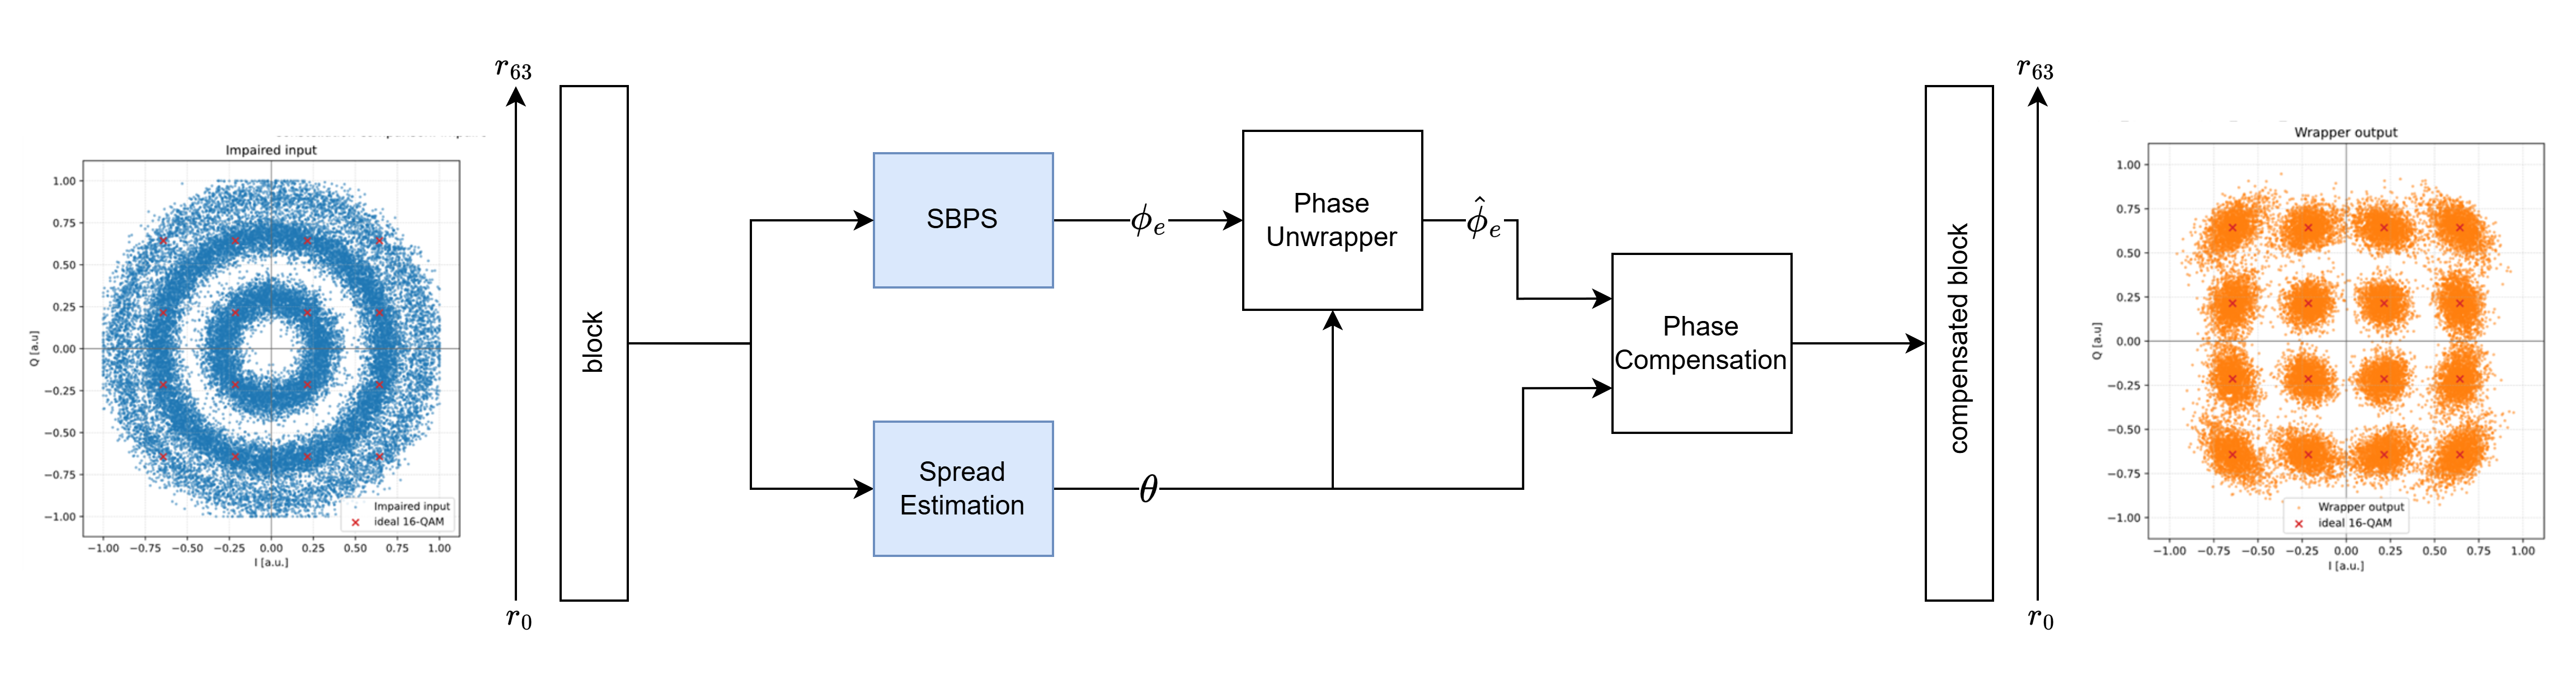
\includegraphics[width=1    \linewidth]{figures/top_architecture.png}
\caption{Top architecture}
\end{figure}
\todo{make figure more clear, seems to minimalistic?}

In the presence of residual \ac{CFO}, the phase evolves approximately linearly with symbol index, while laser phase noise introduces additional random deviations. As a result, a single phase estimate can become insufficient for accurately compensating all symbols inside the block. Symbols located further away from the phase estimation point accumulate additional residual phase error.

The proposed architecture addresses this problem through a two-part carrier recovery structure consisting of:
\begin{enumerate}
    \item a Serialized Blind Phase Search (\ac{SBPS}) block,
    \item and a Spread Estimation (\ac{SE}) block.
\end{enumerate}

The \ac{SBPS} estimates the carrier phase near the middle of the processing block and acts as the central phase reference of the architecture. The \ac{SE} block then estimates how the phase evolves around this midpoint estimate. Rather than estimating a separate phase for every symbol, the architecture reconstructs the intra-block phase evolution from:
\begin{itemize}
    \item one centre-phase estimate,
    \item and one estimate of the total phase spread across the block.
\end{itemize}

This approach is based on the observation that, under practical coherent datacenter operating conditions, the residual \ac{CFO} after coarse frequency recovery dominates the short-term phase evolution within one processing block. The accumulated linewidth-induced phase variation over a single block is typically much smaller than the deterministic phase drift caused by the residual frequency offset:

\begin{equation}
    \sum_{i=0}^{B-1}\phi_i \ll 2\pi \Delta f T_s B
    \label{eq:SE-linear-assumption}
\end{equation}

with $B$ the block size, $\phi_i$ the linewidth-induced phase perturbation of symbol $i$, $\Delta f$ the residual carrier frequency offset and $T_s$ the symbol period.

Under this assumption, the phase evolution across the block may be approximated as locally linear. The carrier phase inside the block can therefore be reconstructed from only:
\begin{enumerate}
    \item the carrier phase near the middle of the block,
    \item and the total phase spread across the block.
\end{enumerate}

Figure~\ref{fig:SBPS-versus-SBPS_and_SE} illustrates the effect that motivates this additional spread estimate. Although the middle of the block can be compensated correctly by the \ac{SBPS} estimate, symbols towards the block edges still exhibit residual constellation rotation when the intra-block phase evolution is ignored.

The estimated spread is subsequently used in two ways:
\begin{enumerate}
    \item to improve phase unwrapping between neighbouring blocks,
    \item and to reconstruct multiple phase corrections within the block during phase compensation.
\end{enumerate}

As a result, the proposed architecture increases the effective frequency tracking range of the carrier recovery system while maintaining substantially lower complexity than conventional high-resolution \ac{BPS} approaches.

%----------------------------------------------------------
% SBPS
%----------------------------------------------------------

\section{Serialized blind phase search}

In a traditional \ac{BPS} implementation, many candidate phases are evaluated simultaneously over the full search interval. For each candidate phase, all symbols inside the processing window are rotated, sliced to the nearest constellation point and evaluated through a decision-directed metric. The candidate yielding the lowest metric is selected as the estimated carrier phase.

For square \ac{QAM} constellations, the search interval may be limited to:

\[
\left[-\frac{\pi}{4},\frac{\pi}{4}\right)
\]

because the \ac{BPS} metric is inherently $\pi/2$-periodic due to the rotational symmetry of square constellations \todo{is source already cited?}.

The key idea of \ac{SBPS} is that the optimal phase estimate is approximated through successive refinement stages. Instead of evaluating many test phases simultaneously, only two candidate rotations are evaluated at each stage:
\begin{itemize}
    \item one positive correction,
    \item and one negative correction,
\end{itemize}
relative to the previously selected estimate.

The candidate producing the lower metric is retained, after which a more refined correction is evaluated during the next stage.

\begin{figure}[H]
\centering
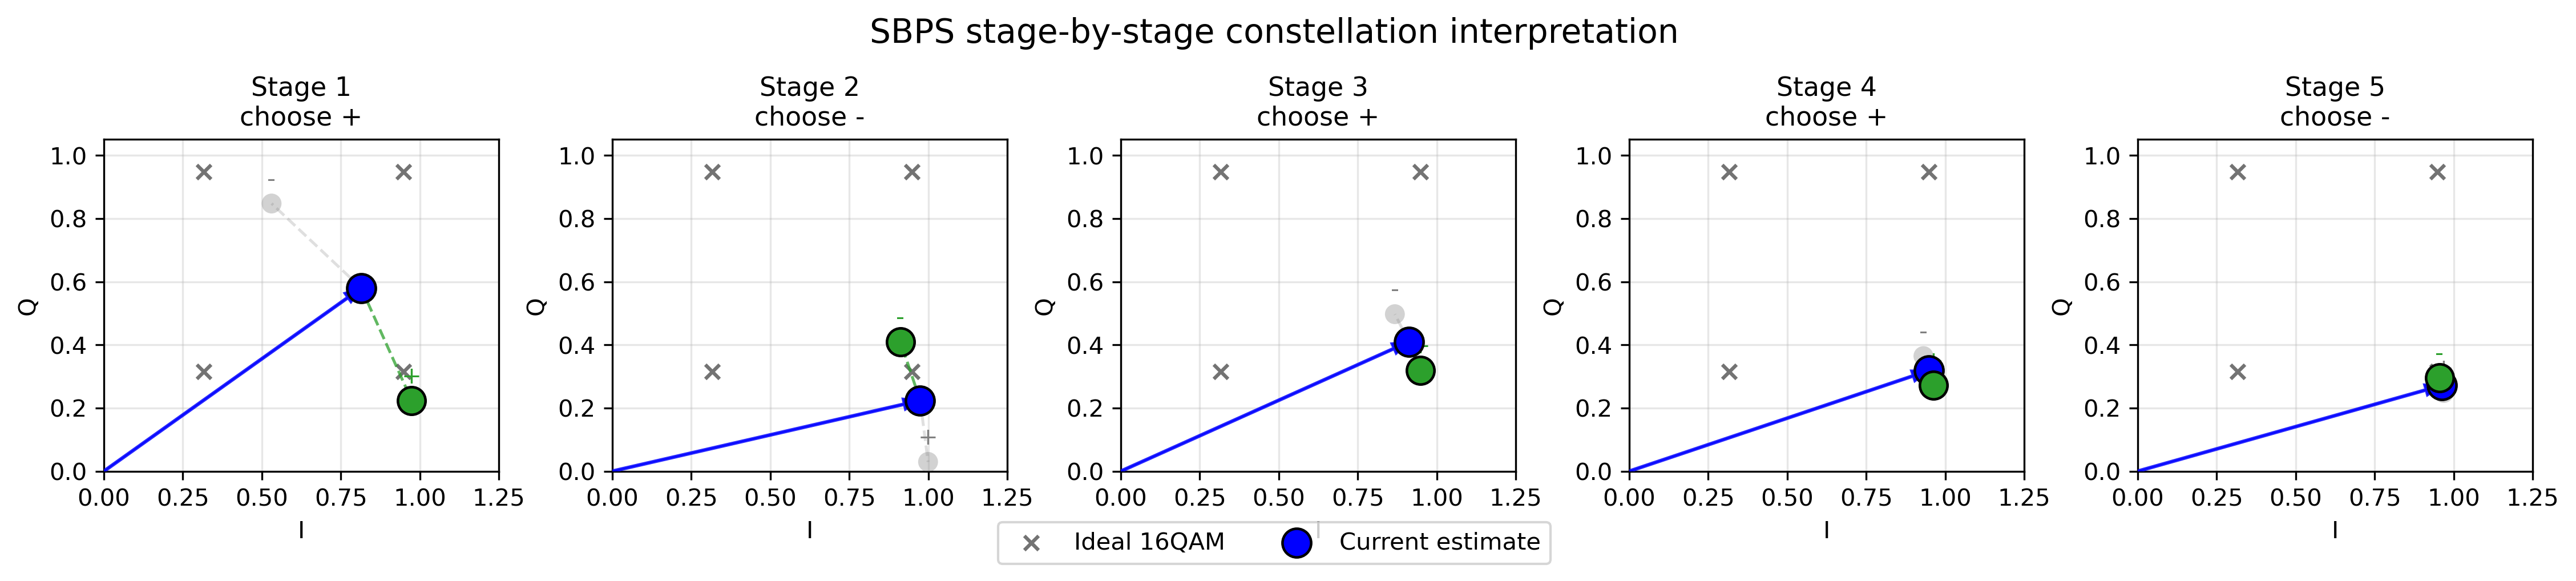
\includegraphics[width=1\linewidth]{figures/sbps_constellation_stages.png}
\caption{Conceptual representation of staged SBPS refinement}
\end{figure}



The proposed implementation adopts a binary refinement structure. The first stage evaluates the hypotheses:

\[
\phi_1 \in
\left\{
-\frac{\pi}{8},
+\frac{\pi}{8}
\right\}
\]

while stage $m$ refines the estimate through:

\[
\hat{\phi}_m
=
\hat{\phi}_{m-1}
\pm
\frac{\pi}{2^{m+2}}
\]

Each stage therefore halves the remaining search uncertainty.

\begin{figure}[H]
\centering
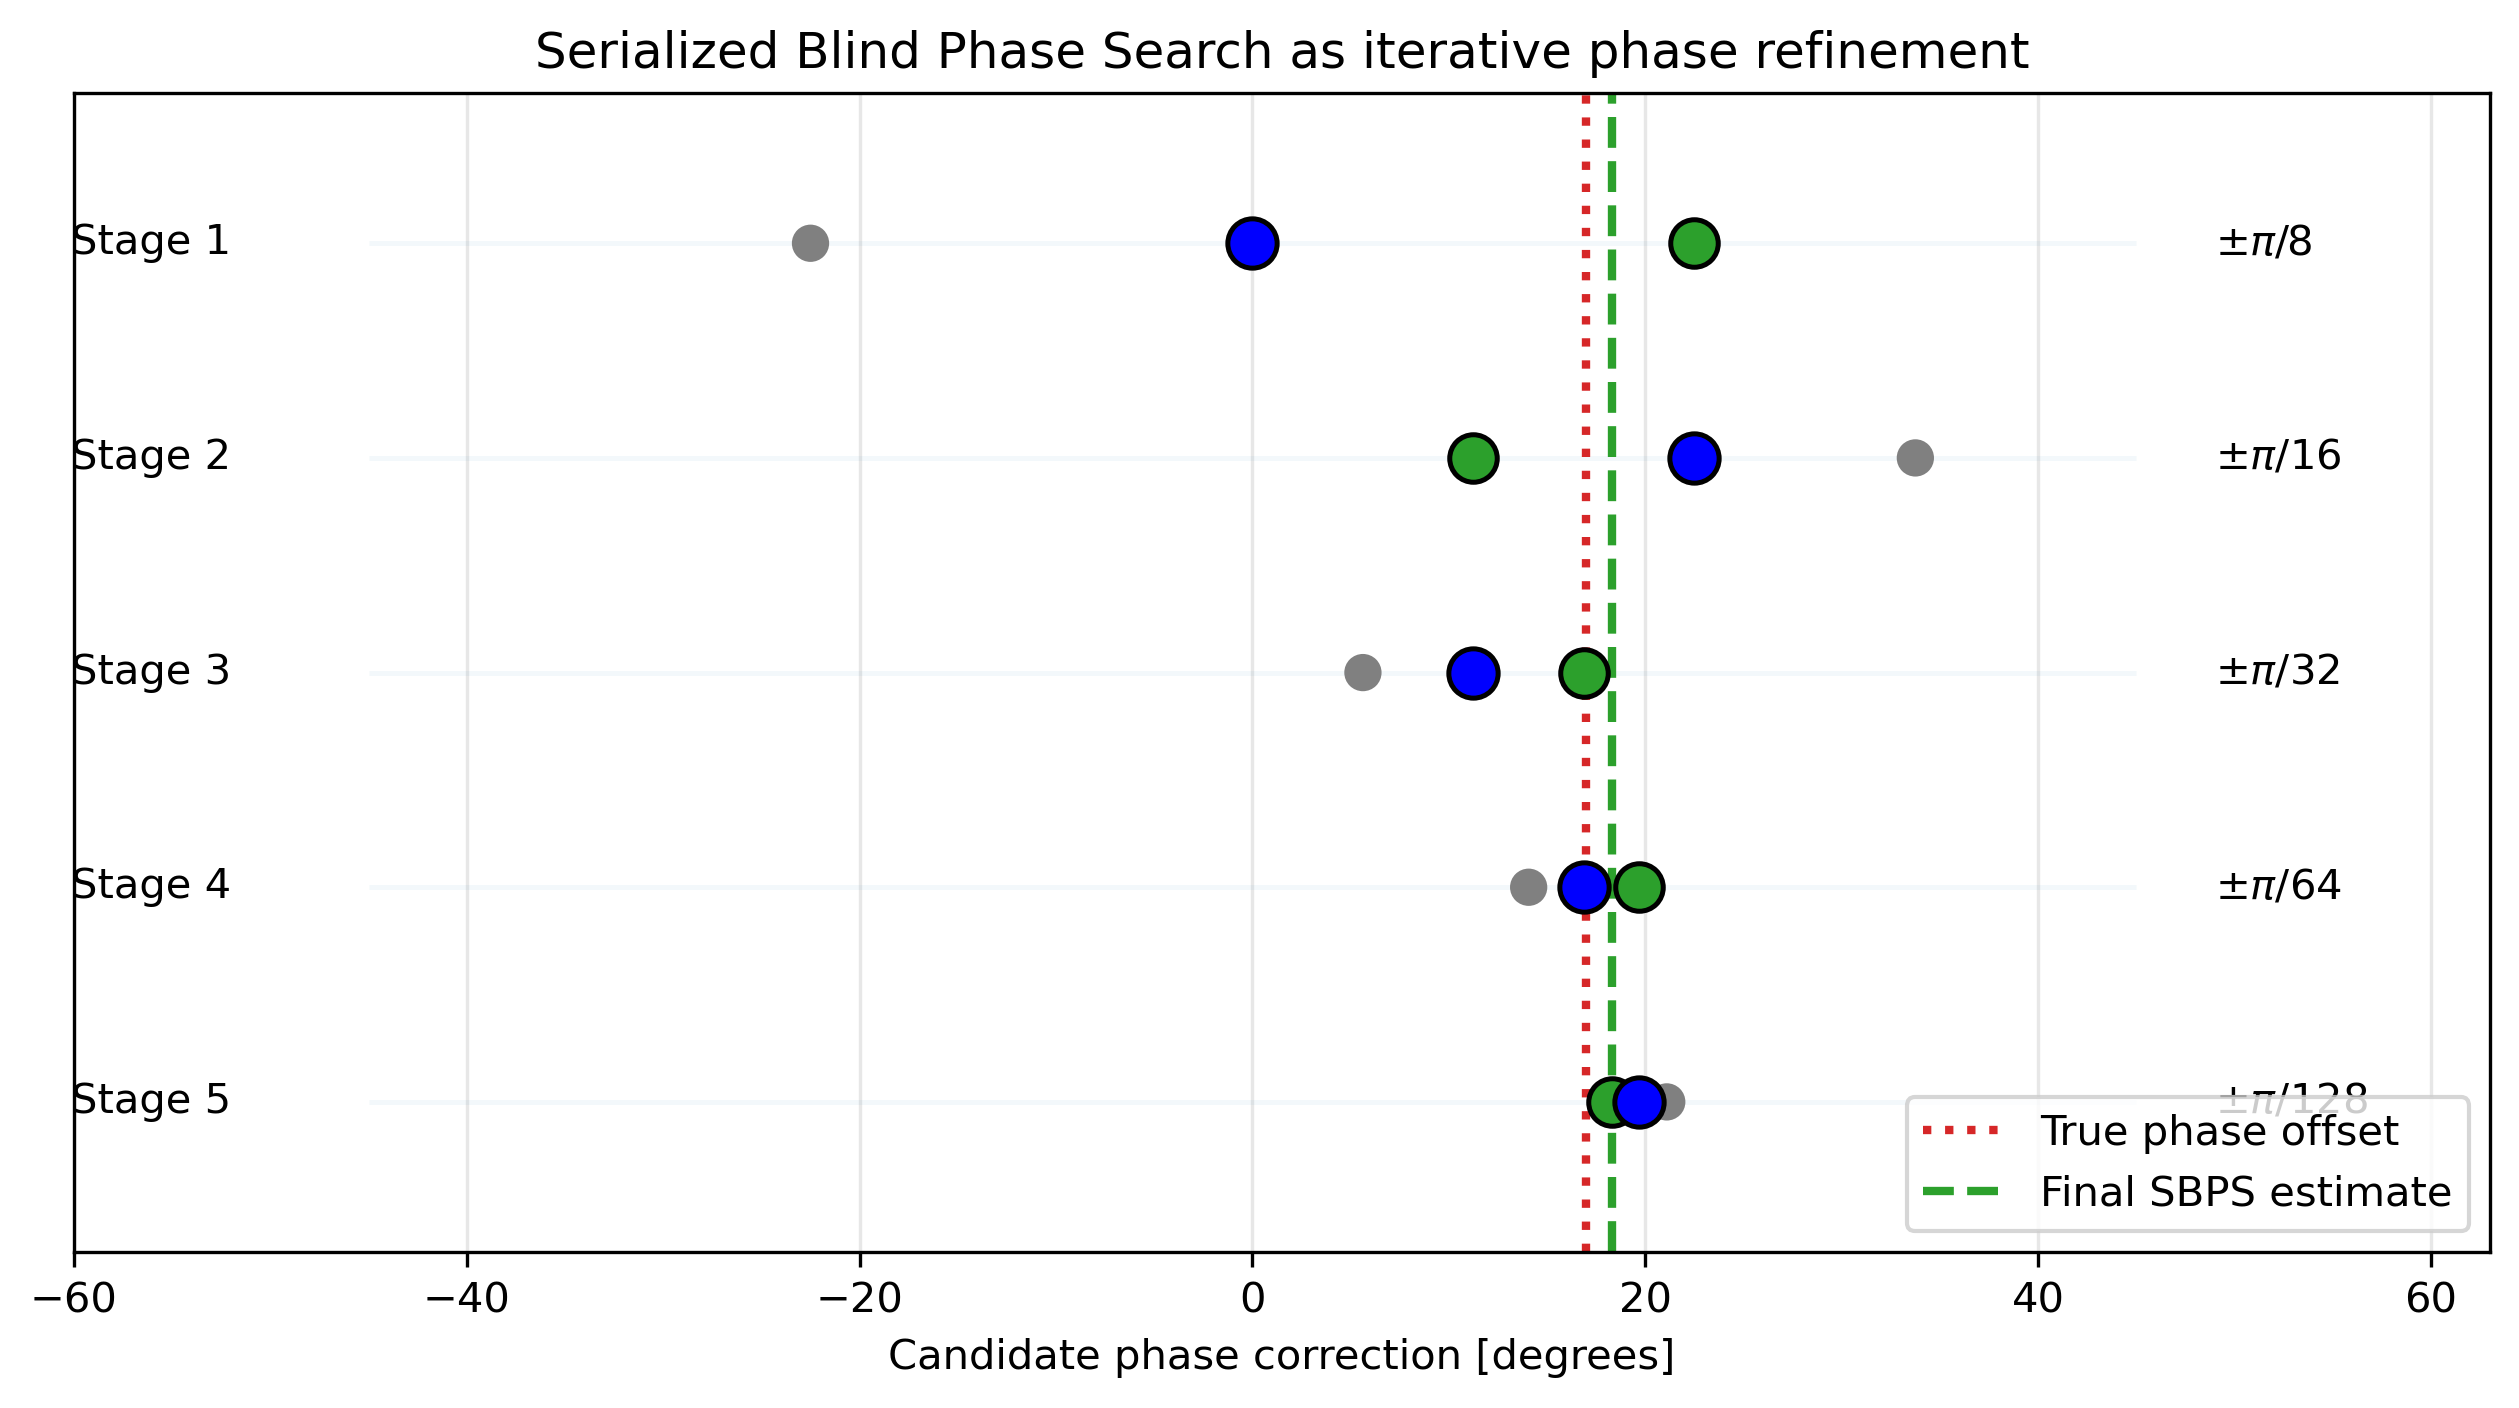
\includegraphics[width=0.8\linewidth]{figures/sbps_phase_refinement.png}
\caption{Phase representation of staged SBPS refinement}
\end{figure}

This procedure is mathematically equivalent to a binary search over the phase interval and yields an exponentially decreasing phase quantization error as the number of stages increases. The referenced work shows that the worst-case estimation error decreases exponentially with each added stage, while the total number of required candidate rotations only increases linearly with the number of stages \cite{Jonas}.

For each candidate phase $\phi$, a decision-directed metric is computed:

\[
J(\phi)=
\sum_{k\in\mathcal{W}}
\left|
D\!\left(r_k e^{-j\phi}\right)
-
r_k e^{-j\phi}
\right|^2
\]

with:
\begin{itemize}
    \item $r_k$ the received symbol,
    \item $D(\cdot)$ the slicer operation,
    \item and $\mathcal{W}$ the metric accumulation window.
\end{itemize}


The candidate phase producing the smallest metric is assumed to correspond most closely to the true carrier phase. In this work, the resulting estimate is interpreted as the carrier phase near the middle of the processing block $ \hat{\phi}_e $.

This estimate is subsequently forwarded to the phase unwrapping and phase compensation stages. Because only one phase estimate is produced per block, and because the \ac{BPS} metric is $\pi/2$-ambiguous for square \ac{QAM} constellations, additional processing is required to track phase continuity between successive blocks. This task is handled by the phase unwrapping stage, while the \ac{SE} block reconstructs the phase evolution inside each block.

\subsection{Block size consideration}

The block size directly influences the effectiveness of the \ac{SBPS} estimate. The coarse frequency recovery stage has a finite \ac{FFT}-bin spacing, which determines the maximum residual \ac{CFO} after frequency recovery. Using the half-bin error bound from Equation~\ref{eq: frequency recovery bin size error}, the residual frequency error satisfies:

\begin{equation}
    \Delta f_e \leq \frac{F_s}{2N_{\mathrm{FFT}}}
\end{equation}

This residual frequency error causes an accumulated phase drift across one \ac{SBPS} processing block of $B$ symbols:

\begin{equation}
    \Delta \phi_{\mathrm{block}} \approx 2\pi \Delta f_e B T_s
\end{equation}

Since $T_s = 1/F_s$, substituting the worst-case residual \ac{CFO} gives:

\begin{equation}
    \Delta \phi_{\mathrm{block,max}}
    =
    2\pi
    \left(
    \frac{F_s}{2N_{\mathrm{FFT}}}
    \right)
    B
    \left(
    \frac{1}{F_s}
    \right)
    =
    \pi\frac{B}{N_{\mathrm{FFT}}}
\end{equation}

The worst-case accumulated phase drift over one block therefore depends on the ratio between the processing block size and the \ac{FFT} size, and not directly on the sampling frequency. For an unwrapping threshold of $\pi/4$, the phase drift over one block should satisfy:

\begin{equation}
    \Delta \phi_{\mathrm{block,max}} \leq \frac{\pi}{4}
\end{equation}

which yields the design condition:

\begin{equation}
    N_{\mathrm{FFT}} > 4B
\end{equation}

For example, a block size of $B = 64$ requires at least $N_{\mathrm{FFT}} > 256$ to avoid additional cycle slips from the worst-case coarse frequency recovery error. This is only a theoretical minimum. In practice, a margin is required because linewidth-induced phase noise, additive noise and estimation errors also affect the phase trajectory.

The block size also creates a trade-off in estimation quality. A larger metric accumulation window improves robustness against additive noise because random perturbations are averaged over more samples \cite{Mello_2018}. At the same time, a larger block spans a longer time interval, so the carrier phase variation caused by residual \ac{CFO} and laser phase noise becomes larger within the block. This trade-off is one of the main motivations for combining a middle-block \ac{SBPS} estimate with a separate \ac{SE} block.

%----------------------------------------------------------
% SPREAD ESTIMATION
%----------------------------------------------------------

\section{Spread estimation algorithm}

As discussed in Sections~\ref{phase noise and frequency offset} and~\ref{carrier recovery in DSP chains}, the residual impairments after coarse frequency recovery consist of both stochastic laser phase noise and a remaining carrier frequency offset. While the linewidth-induced phase noise behaves as a random Wiener process, the remaining frequency offset introduces an approximately linear phase ramp across a processing block, as illustrated in Figure~\ref{fig:linear_approx}.

The proposed \ac{SBPS} architecture estimates only a single carrier phase per block, namely the phase located near the middle of the block. This estimate is sufficiently accurate to serve as a robust phase reference for the block as a whole, but it does not describe how the phase evolves within the block itself. As a result, directly compensating all symbols using only the middle-block phase estimate still leaves a residual phase error on symbols located further away from the block centre.

This effect becomes increasingly important when the residual \ac{CFO} after frequency recovery becomes larger, when the processing block size increases or when the laser linewidth introduces additional phase drift.

\begin{figure}[H]
\centering
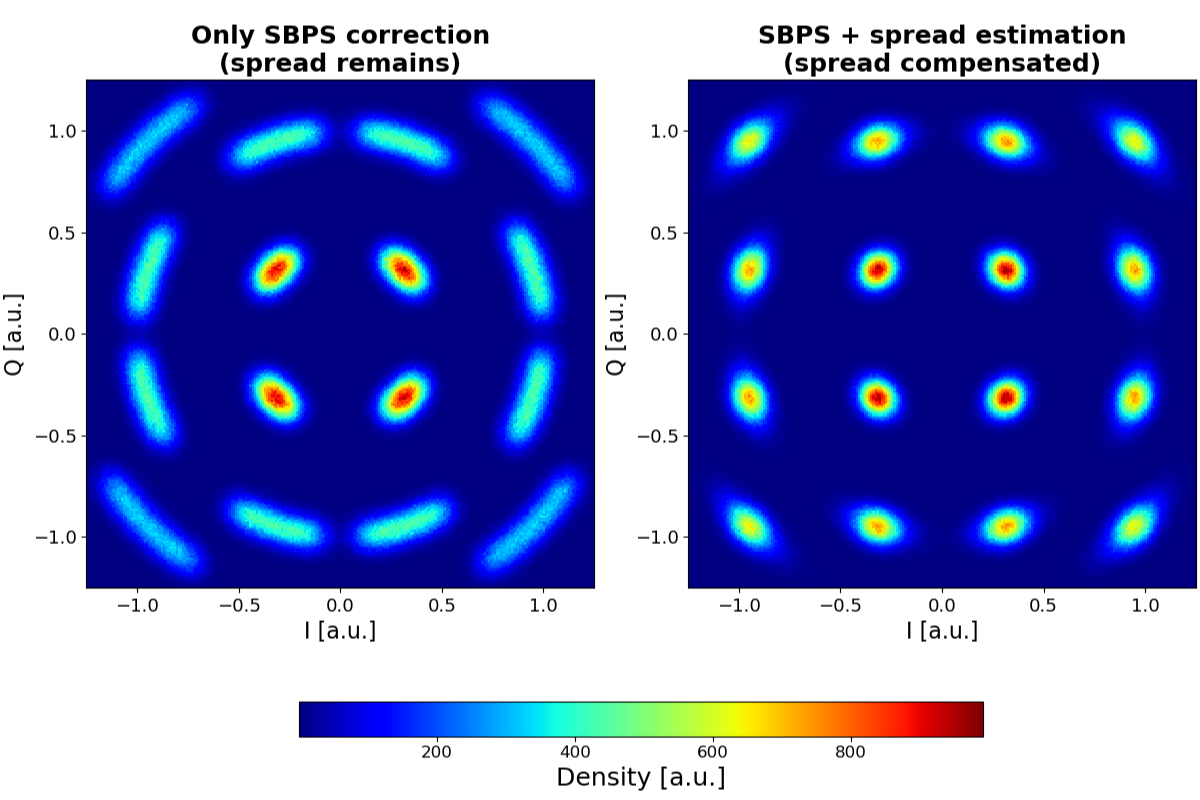
\includegraphics[width=0.8\linewidth]{figures/SBPS_versus_SBPS+SE_correction.png}
\caption{Residual phase correction with SBPS only and with combined SBPS+SE correction}
\label{fig:SBPS-versus-SBPS_and_SE}
\end{figure}

The \ac{SE} block is introduced to estimate this residual phase evolution across the block. Rather than estimating a separate carrier phase for every symbol, which would significantly increase computational complexity, the proposed method estimates the total phase spread over the block and reconstructs the intermediate phase trajectory from this information.

The proposed spread estimation algorithm operates on symbols that are raised to the fourth power. For square \ac{QAM} constellations, the fourth-power operation suppresses the modulation-dependent phase terms while preserving the carrier-related phase rotation.

For a received symbol:

\begin{equation}
r_k = a_k e^{j\phi_k}
\end{equation}

the fourth-power operation gives:

\begin{equation}
r_k^4 = a_k^4 e^{j4\phi_k}
\end{equation}

The modulation phase ambiguity is removed because square \ac{QAM} constellations exhibit rotational symmetry over multiples of $\pi/2$. After fourth-power transformation, the dominant remaining phase term therefore corresponds to four times the underlying carrier phase evolution.

Under the locally linear phase assumption introduced in Equation~\ref{eq:SE-linear-assumption}, the total phase spread across the block may be estimated from representative symbols located near:
\begin{itemize}
    \item the beginning of the block,
    \item the middle of the block,
    \item and the end of the block.
\end{itemize}

The first and last symbols are used to estimate the magnitude of the total phase spread, while the middle symbol assists in determining the direction of the phase evolution.

Let $R_0$ and $R_{B-1}$ denote the selected fourth-power symbols near the beginning and end of the block. The cosine of the total phase spread may then be estimated through the normalized dot product:

\begin{equation}
\frac{\langle R_0,R_{B-1}\rangle}
{\|R_0\|\|R_{B-1}\|}
=
\cos(4|\theta|)
\label{eq:spread-cos}
\end{equation}

with $\theta$ the total phase spread across the block.

The spread magnitude can therefore be recovered through:

\begin{equation}
|\theta| =
\frac{1}{4}
\arccos
\left(
\frac{\langle R_0,R_{B-1}\rangle}
{\|R_0\|\|R_{B-1}\|}
\right)
\label{eq:spread-mag}
\end{equation}

The use of $\arccos(\cdot)$ instead of $\arctan(\cdot)$ is important because the total phase spread may exceed $\pi$. A direct arctangent-based angle estimation could therefore lead to sign ambiguities and incorrect unwrap decisions. The cosine-based formulation instead estimates only the absolute spread magnitude, after which the spread direction is estimated separately.

To determine the direction of the phase evolution, a second estimate is performed using symbols from the beginning and middle of the block. The sign of the phase evolution can be obtained through the sign of the complex cross product:

\begin{equation}
\mathrm{sign}(\gamma)
=
-\mathrm{sign}
\left(
\Re\{R_0\}\Im\{R_b\}
-
\Im\{R_0\}\Re\{R_b\}
\right)
\label{eq:spread-sign}
\end{equation}

with $R_b$ the selected middle-region symbol.

Combining both estimates yields the final spread estimate:

\begin{equation}
\hat{\theta}
=
\mathrm{sign}(\gamma)
\cdot
|\theta|
\label{eq:spread-final}
\end{equation}

The estimated spread is subsequently used to extrapolate leading and lagging phase estimates for the phase unwrapper and to reconstruct multiple phase corrections inside the block during phase compensation.

The method nevertheless introduces several limitations specific to square 16QAM constellations. Unlike \ac{QPSK}, where the fourth-power operation maps all transformed symbols onto a single radius, the fourth-power transformation of 16QAM results in multiple amplitude rings. Some transformed constellation points therefore become unsuitable for accurate spread estimation because their relative phase relationships introduce ambiguities.

As a consequence, not every received symbol may be used directly for spread estimation. The architecture therefore includes an input-selection stage that identifies suitable candidate symbols before the actual spread calculation is performed.

\subsection{Input symbol consideration}\label{input selector}

For \ac{QPSK}, the fourth-power operation maps all constellation symbols onto a single circle. For square 16QAM, however, the transformed symbols occupy multiple radii after the fourth-power operation. This behaviour is illustrated in Figure~\ref{fig:fourth-power-constellation}.

\begin{figure}[H]
\centering
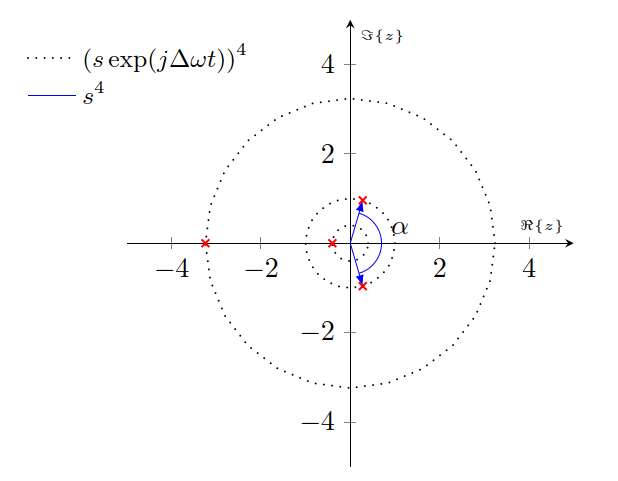
\includegraphics[width=0.45\linewidth]{figures/symbols_to_fourth_power.png}
\caption{16QAM symbols after fourth-power transformation}
\label{fig:fourth-power-constellation}
\end{figure}
\todo{find more representative mapping}


Symbols originating from the middle ring of the 16QAM constellation can introduce large phase ambiguities after fourth-power transformation. Using these symbols directly in the normalized dot-product calculation of Equation~\ref{eq:spread-cos} can therefore lead to incorrect spread estimates. To mitigate this problem, the spread estimator only considers symbols originating from the inner and outer constellation rings. These symbols retain an unambiguous phase transformation after the fourth-power calculation and therefore yield more reliable spread estimates.

Rather than searching the complete processing block for suitable symbols, only a limited subset of symbols near the beginning, middle and end of the block is evaluated. This reduces hardware complexity while maintaining a sufficiently high probability of finding valid candidate symbols.

Let $N$ denote the number of candidate symbols evaluated per region. Assuming uniformly distributed 16QAM symbols, the probability of finding at least one valid candidate pair may be approximated by:

\begin{equation}
P(\mathrm{hit})
=
1 -
\left[
\left(
\frac{1}{2^N}
\right)^2
+
2
\left(
\frac{1}{2^N}
\left(
1-\frac{1}{2^N}
\right)
\right)
\right]
\label{eq:selection-prob}
\end{equation}

A moderate value of $N$ therefore already yields a high probability of obtaining usable symbols while avoiding the hardware cost associated with a full-block search. For example, $N=3$ gives $P(\mathrm{hit}) = 49/64 \approx 76.6\%$ under the uniform-symbol assumption. If no suitable candidate combination is found, the previously estimated spread value is retained. This behaviour is justified by the relatively slow variation of practical laser frequency offsets compared to the short duration of a processing block in baudrate-sampled coherent systems.

The selected candidate symbols are subsequently forwarded to the hardware blocks responsible for fourth-power calculation, spread estimation and sign estimation.

\section{Phase unwrapping}
\section{Phase compensation}

\section{Expected performance}



